

% \subsection{Synthetic benchmark networks}
% One important finding in~\cite{nicolini2016} is that brain networks are organized in modules with heterogeneous size distributions.
% We implemented this property in our two types of benchmark networks.
% For the first test, we generated a ring of cliques with $300$ nodes, and sizes of the cliques sampled from a power-law with exponent $\tau_c=2$, minimum and maximum clique size respectively $\min_c=5$, $\max_c=50$ (see also Supplementary Materials S4).
% For each subject of the sample, we synthesized $150$ time-points for each node using the \texttt{neuRosim R} package~\cite{neurosim2011}.
% We set the baseline value of all the time series to $100$~\cite{welvaert2013}.

% Finally, we correlated the original synthetic time series $\mathbf{X}$ by multiplication with the matrix $\mathbf{L}$, obtained the correlated time series $\mathbf{Y}$ and added Rician noise~\cite{Gudbjartsson1995} to $\mathbf{Y}$ independently for each area. The simulated data $\mathbf{Y}$ did not include slow drift components, simulated physiological noise, nor spatial noise. The average SNR was defined as $\textsc{SNR}=\bar{S}/\sigma_N$ where $\bar{S}$ is the average magnitude of the signal and $\sigma_N$ is the standard deviation of the noise~\cite{kruger2011}.

% In order to be more exhaustive and extend the validity of results, we repeated the same procedure on weighted LFR networks with $N=600$ nodes, sampling nodes degree from a power-law with exponent $\tau_d=2$, average degree $\left<k\right>=12$ and maximum degree $\max_k=50$.
% We set the topological and weights mixing coefficients, i.e. the average fraction of intra-cluster and inter-cluster degree and strengths, to $\mu_t=0.1$ and $\mu_w=0.1$, respectively. Planted community sizes ranged from $5$ to $50$ nodes and were sampled from a power law with exponent $\tau_c=1$. In the Supplementary Information we have extended this analysis to a wider range of network parameters.

% Group-level correlation matrices were computed by Fisher-transforming and averaging individual instances of the above matrices. Sparsification was obtained by removing edges with weights below the most stringent threshold that maintained the network connectedness, a procedure known as percolation analysis~\cite{gallos2012,bardella2016a,alexander-bloch2010}. This approach measures the size of the largest connected component of the network upon iterative removal of the weakest edges and enables data-driven determination of the optimal sparsification threshold that preserves network structure and connectedness while removing potentially spurious correlations.

% The community structure of the resulting weighted sparsified matrices was detected by Asymptotical Surprise optimized with PACO and compared against two widely used methods, Infomap~\cite{rosvall2008} and Newman's Modularity~\cite{blondel2008,newman2006}, that are affected by the resolution limit, albeit to different extents. 
% In Newman's Modularity, the size of the smallest detectable cluster is of the order of the square root of the number of edges in the entire network~\cite{fortunato2007}, while Infomap has a limit that depends on the overall number of inter-cluster edges~\cite{kawamoto2015}.
% Here we used the Louvain implementation available in the Brain Connectivity toolbox~\cite{rubinov2010} and the Infomap implementation available in the \texttt{igraph-0.7.1} package~\cite{igraph2006}.

% For all methods, including PACO, we launched $10,000$ independent runs, and picked the membership corresponding to the partition with the best value of the fitness function, the maximum for Modularity and Asymptotical Surprise, the minimum for Infomap.

% As discussed in the previous chapter, sections~\ref{sec:degeneracy},~\ref{sec:degeneracy_surprise},~\ref{sec:degeneracy_asymptotical_surprise}, degeneracy of nearly-optimal solutions does not appear to severely affect Surprise or Asymptotical Surprise, and a consensus approach is not deemed necessary for these functions.
% This analysis supports our choice to select the solution with the highest value of the fitness function.

% \subsection{Measures of partition quality}
% For each method, we analyzed the level of agreement of the detected community structure against the planted one in terms of Normalized Mutual Information (NMI)~\cite{danon2005}.
% Additionally, we used two different coefficients of similarity between partitions: Sensitivity and Specificity. 

% To this end, we quantified the confusion matrix $\mathbf{C}$ between the detected and planted modules. Each element $C_{ij}$ is the number of nodes in the planted community $i$ that appear in the detected community $j$.
% For each planted community we scored as true positives (TP) the nodes correctly identified as belonging to the ground-truth community, and as false positives (FP) the nodes wrongly assigned to a community; similarly false negatives (FN) were nodes wrongly classified in different communities and true negatives (TN) the nodes correctly classified as out of the community.
% Sensitivity, defined as $TP/(TP+FN)$, decreases with increasing number of False Negatives. Specificity instead is defined as $TN/(TN+FP)$ and decreases when many nodes are wrongly assigned in the same community.
% Additionally, we computed Accuracy and Matthew Correlation Coefficient (see Supplementary Materials for definitions)\todo{mettere definizioni matthew correlation coefficient}.

% % \subsection{Human resting state network}
% % We applied Asymptotical Surprise maximization by PACO to the same reference resting state fMRI functional connectivity dataset from healthy subjects~\cite{crossley2013a} as described previously in section~\ref{sec:surprise_optimization_fc_networks}.

% \subsection{PACO benchmark on synthetic networks}
% We compared the quality of the partitions of the synthetic benchmark networks obtained by Asymptotical Surprise with those of Infomap~\cite{rosvall2008} and Newman's Modularity ~\cite{newman2006,blondel2008}. Figure \ref{fig:nmisensitivityspecificityringclique} shows Normalized Mutual Information, Sensitivity and Specificity of the three methods applied to the ring of cliques for different sample sizes and SNRs; no-noise condition is represented as ``Inf''.
% This model network was constructed to test the ability of the three methods to retrieve heterogeneous community structures under various noise conditions.

% As expected, all methods showed better performance with increasing SNR and number of subjects, as noise and intersubject variability introduce spurious edges that hinder the ability to retrieve the planted structure.
% Partitions obtained with Newman's modularity showed the lowest NMI with respect to the planted partition under all conditions.
% Sensitivity of Newman's modularity did not exceed $0.75$ even for high SNRs and a large number of subjects, a consequence of its stronger resolution limit.
% For this network, Infomap performed substantially better in terms of NMI against the planted partition, with a Sensitivity that was superior to that of Modularity across the spectrum of conditions.

% Asymptotical Surprise showed highest NMI and Sensitivity across conditions, consistent with its resolution-limit-free behavior.
% Asymptotical Surprise proved superior in terms of NMI and Sensitivity in the low SNR regimes, and in the presence of relatively large intersubject variability as mimicked by the generation of different instances of the ring of cliques (see Methods section).
% Specificity of Asymptotical Surprise was not inferior to the other methods under all conditions, thus ruling out increased vulnerability to False Positives, at least in this particular model network.

% \begin{figure}[htb!]
% 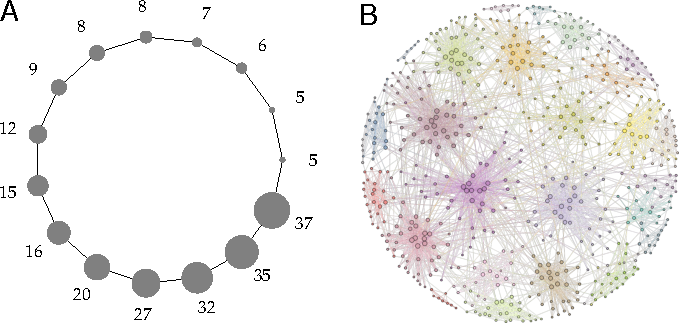
\includegraphics[width=1\textwidth]{images/pacopaperfigure1.pdf}
% \caption{The two benchmark networks used in this study, laid out. (A) is a power-law ring of cliques, where cliques present different sizes sampled from a power-law distribution;
% (B) is the layout of an LFR network with parameters $N=600$, $\left< k \right>=12$, $\max_k=50$, $\mu_t=0.1$, $\mu_w=0.1$, $\min_c=5$, $\max_c=50$.
% The layout of (B) was generated with the graph-tool library~\cite{peixoto_graph_tool_2014}.}
% \label{fig:lfrringclique}
% \end{figure}

% \begin{figure}[htb!]
% 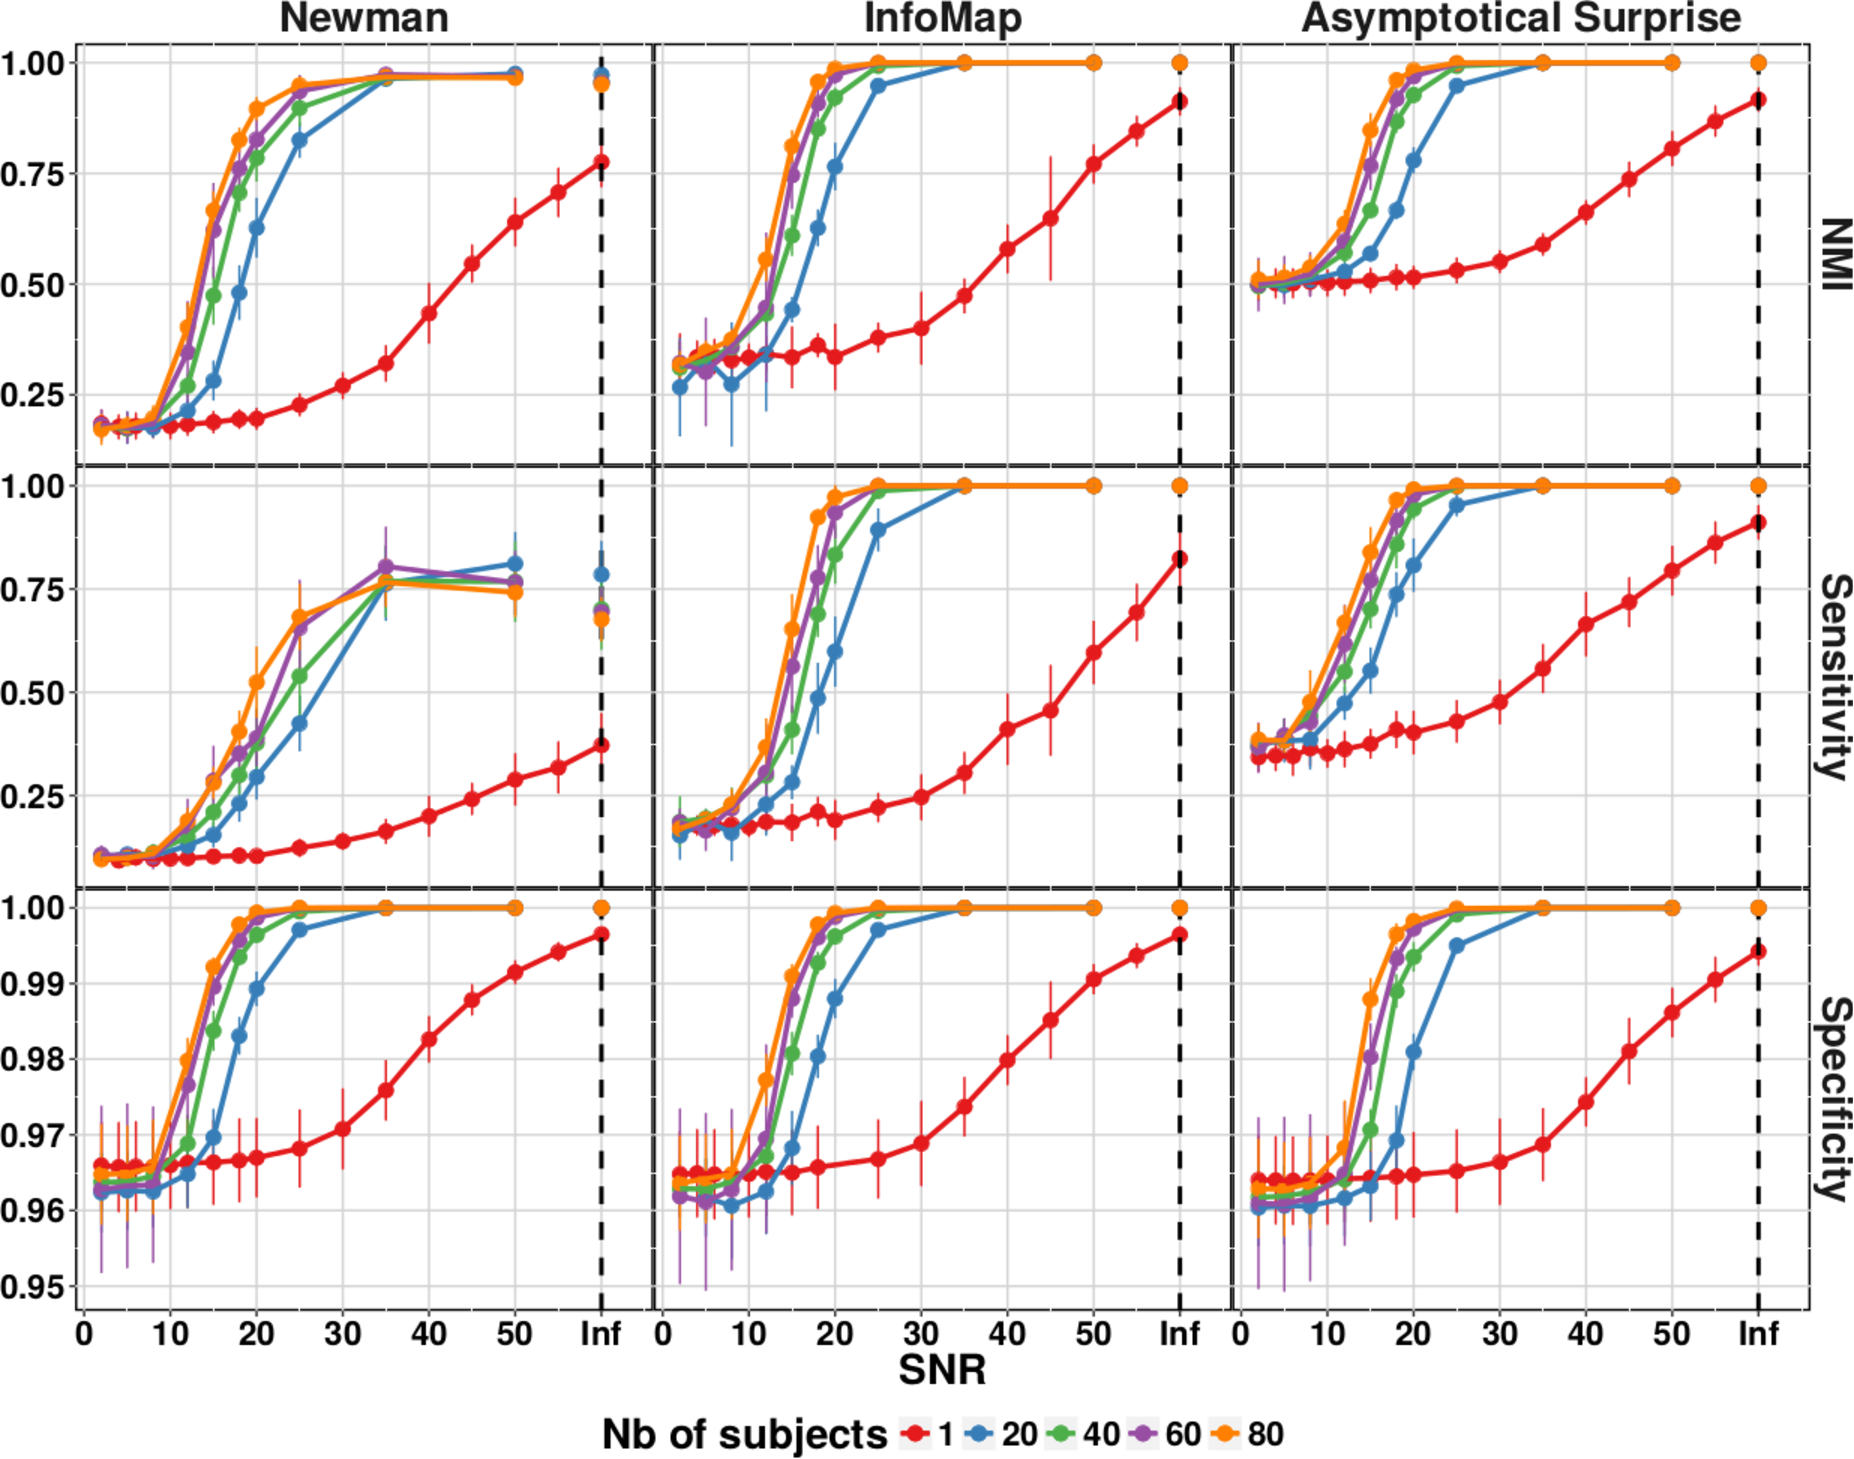
\includegraphics[width=\textwidth]{images/pacopaperfigure4.pdf}
% \caption{NMI, Sensitivity and Specificity of the three community detection algorithms applied to a power-law ring of clique network. SNR indicates Signal to Noise Ratio, and Inf the situation with a network structure unperturbed by noise. Number of Subjects indicates the different number of instances used to generate the group level network.}
% \label{fig:nmisensitivityspecificityringclique}
% \end{figure}

% Comparable results were obtained for the LFR network (Figure~\ref{fig:nmisensitivityspecificitylfr}), a model graph that replicates the distribution of nodal degree observed in many real-world networks, including those representing brain functional connectivity.
% All three methods showed similar values of NMI for high SNR and a large number of subjects, with a plateau reaching maximum Sensitivity with a group sample bigger than $20$ and SNR above $30$.
% Sensitivity was only slightly worse for Modularity, but it should be noted that for the LFR network the size distribution of the planted modules was narrower than for the ring of cliques (Figure~\ref{fig:lfrringclique}), thus making the resolution limit less evident.

% \begin{figure}[htb!]
% 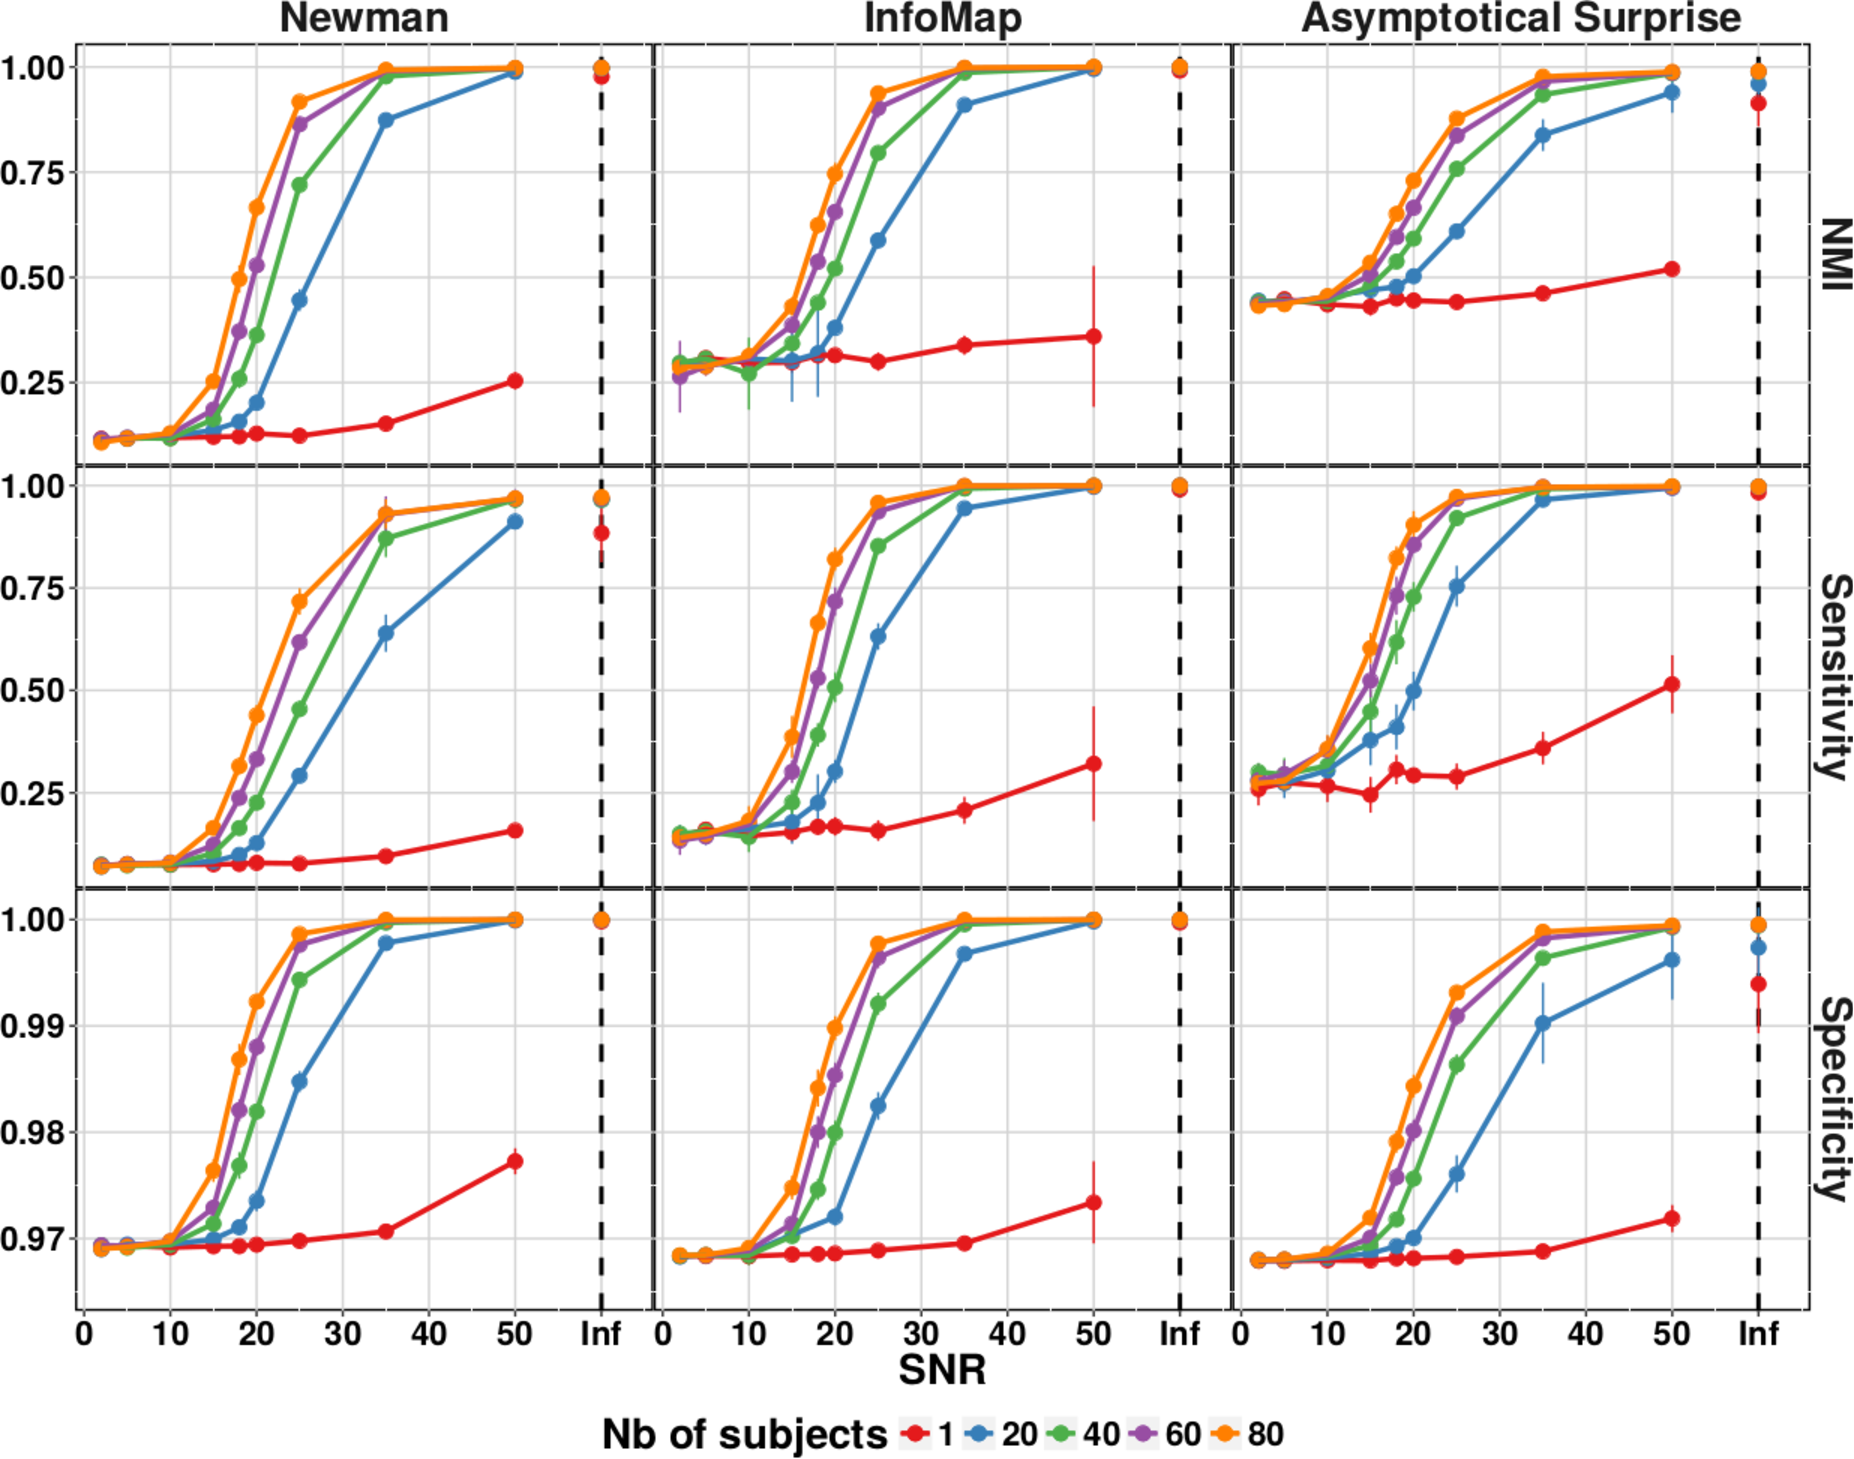
\includegraphics[width=\textwidth]{images/pacopaperfigure5.pdf}
% \caption{NMI, Sensitivity and Specificity of the three community detection algorithms applied to Lancichinetti-Fortunato-Radicchi (LFR) networks. SNR indicates Signal to Noise Ratio, and Inf the situation with a network structure unperturbed by noise. Number of Subjects indicates the different number of instances used to generate the group level network.}
% \label{fig:nmisensitivityspecificitylfr}
% \end{figure}

% In the lower SNR regime, Asymptotical Surprise presented the best performance in terms of NMI and Sensitivity, with a slower decay for decreasing SNR. 
% Specificity was almost equivalent across the three methods, with a quick convergence to the maximum value of 1 for high SNR and good performance (around $0.97$) for low SNR.
% Asymptotical Surprise presented a faster decay with decreasing SNR.
% However, it should be noticed that the scale of Specificity has a very narrow range ($0.97$-$1.00$), and the differences between the three methods were relatively small.

% Consensus analysis applied to Newman's Modularity to assess the potential effects of the degeneracy of nearly optimal solutions did not show substantial differences in the comparison with the other methods (Supplementary Information, Figure S6, S7).

% For the sake of completeness, we also computed Accuracy and Matthew Correlation Coefficient for the same model networks, shown in the Supplementary Materials.
% Notably, Infomap showed a large variability in Accuracy for lower SNRs and number of subjects.
% Under closer examination, however, it appeared that the increased variance for Infomap was due to occasional runs in which the algorithm only retrieved one or two large modules.
% This is a known problem with Infomap and other algorithms based on random walks that depends on the need to parametrize the teleportation step in order to make the dynamics ergodic~\cite{lambiotte2012}.

% Altogether, the picture that emerges from the analysis of Accuracy and MCC is entirely consistent with the results shown in this section.

% \subsection{Asymptotical Surprise on resting state dataset}
% Figure~\ref{fig:partitioncomparison} shows a comparison between the modular structure of the resting state fMRI dataset obtained with Newman's Modularity, Infomap and Asymptotical Surprise.
% For each method, we had $10,000$ independent runs and picked the partition with the best value of the respective fitness functions ($Q=0.4967$, $\mathcal{L}=8.5173$, $S_a=5925.3$, for Modularity, Infomap and Asymptotical Surprise, respectively).
% The three methods showed significantly different partitions (relative NMIs in Table 1), with a number of detected communities of 10, 19 and 47 for Modularity, Infomap and Asymptotical Surprise, respectively.
% Interestingly, Modularity detected a relatively uniform size distribution, consistent with the intrinsic scale built into the fitness function.
% Infomap showed a wider distribution of module sizes, with number of nodes ranging between 156 and 3, while Surprise showed the largest spread, and included communities as small as single nodes (singletons).

% \begin{figure}[htb!]
% 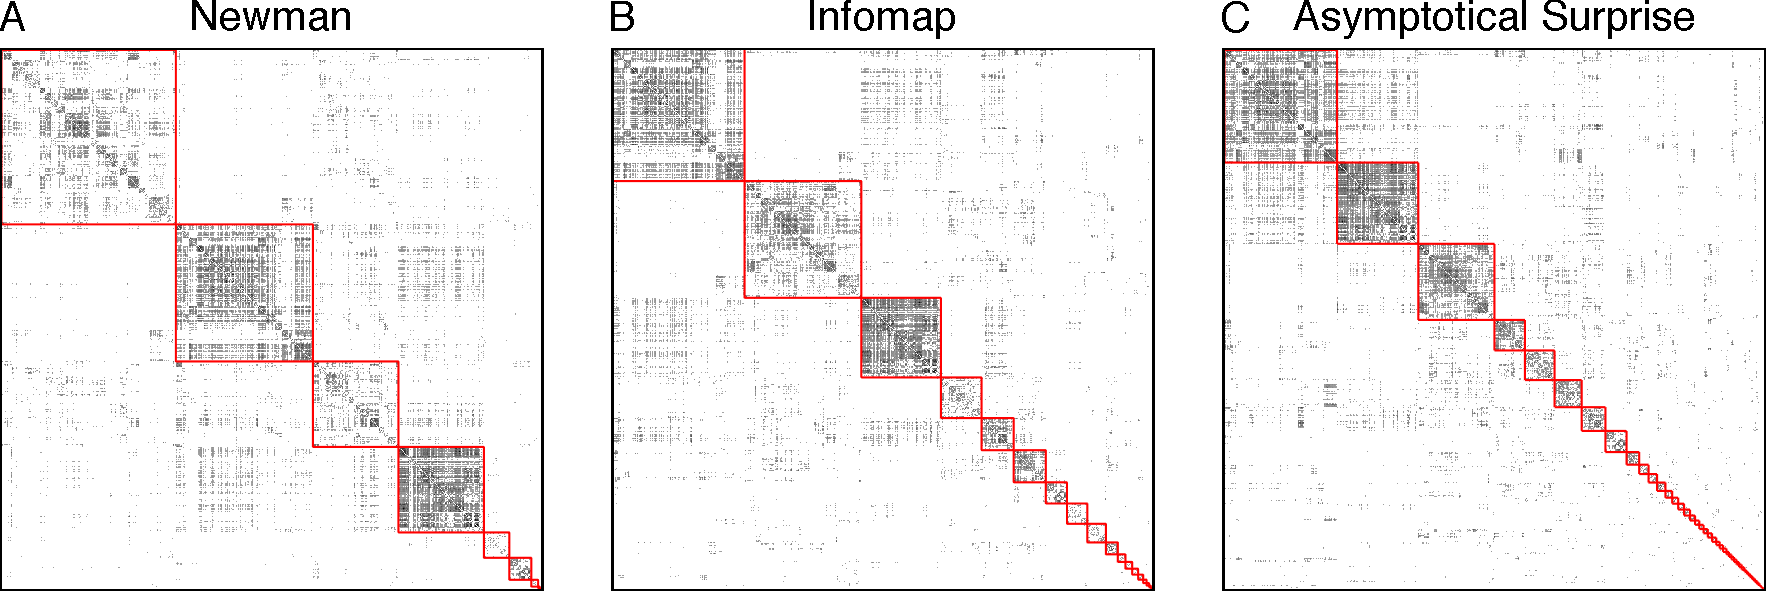
\includegraphics[width=\textwidth]{images/pacopaperfigure6.pdf}
% \caption{Adjacency matrix of the resting state functional connectivity network. The node indices have been reordered by module membership in each graph, and the red lines highlight the community structures obtained by A) Louvain-Newman's Modularity ($Q=0.4967$); B) Infomap ($L=8.5173$); C) Asymptotical Surprise ($S_a=5925.28$).}
% \label{fig:partitioncomparison}
% \end{figure}


% Figure~\ref{fig:cervellini4x4} shows the 16 largest modules detected by Asymptotical Surprise, ranked by number of nodes comprised in each community. 
% The first and largest module (Fig. \ref{fig:cervellini4x4}A) includes the pre- and post-central gyri, part of the supramarginal gyrus and supplementary motor area.
% The second community (Fig. \ref{fig:cervellini4x4}B) consists largely of nodes belonging to the occipital lobe: the visual areas and the surrounding calcarine sulcus, the lingual and fusiform gyrus.
% The third module (Fig. \ref{fig:cervellini4x4}C) reflects the Default Mode Network, spanning the temporo-parietal cortex, the medial prefrontal cortex and the posterior cingulate/precuneus.
% The nodes involved in the executive frontal functions form the fourth largest community.
% Interestingly, nodes in the communities D, E, G are the major players that take part in the so-called fronto parietal attentional network~\cite{markett2014}.
% The auditory network, comprising temporal areas, was detected as a distinct community (Fig. \ref{fig:cervellini4x4}F).
% Deeper structures emerge as separate modules in Fig. \ref{fig:cervellini4x4}H, with subcortical areas including the basal ganglia, i.e. putamen, globum pallidum, caudate nucleus and the whole thalamus.
% The hippocampus and the parahippocampal gyrus were identified as separate communities (O and P).
% Additional, smaller substructures are shown in the third and fourth row of Figure~\ref{fig:cervellini4x4}, including the Supplementary Motor Area (Fig. \ref{fig:cervellini4x4}J) and the orbital (Fig. \ref{fig:cervellini4x4}M) and orbitofrontal (Fig. \ref{fig:cervellini4x4}I) modules, containing nodes from Brodmann area 47 (the smaller communities are displayed Figure S8).

% \begin{figure}[htb!]
% \includegraphics[width=\textwidth]{images/pacopaperfigure7.pdf}
% \caption{Sixteen largest modules found by Asymptotical Surprise Maximization in the resting state network overlaid on an MRI brain template. The modules are ranked by decreasing size, and named after corresponding functional networks previously identified by multivariate analysis of resting state fMRI data, or by the comprised anatomical districts.}
% \label{fig:cervellini4x4}
% \end{figure}

% Partitions of the functional connectivity network obtained by Newman's Modularity and Infomap are reported in the Supplementary Materials Section (Figures S9 and S10).
% Newman's Modularity retrieved four large, relatively uniform communities, corresponding to the Default Mode Network, the central network, occipital and frontoparietal networks.
% This is in keeping with previous studies using Modularity optimization by spectral decomposition~\cite{crossley2013a}, and consistent with the strong resolution limit that affects this method.
% Additionally, a few smaller modules were found by Louvain optimization of Newman's Modularity, corresponding to the basal ganglia, the hippocampal/parahippocampal formation and two asymmetrically distributed subcortical clusters.

% Infomap identified 19 communities of various sizes, also shown in the Supplementary Materials Section, Figure S10.
% The largest modules showed a close correspondence with those identified by Asymptotical Surprise, albeit with some notable differences.
% By way of example, the largest component includes the motor-sensory and auditory modules, identified as separate communities by Asymptotical Surprise.
% The Default Mode Network retrieved by Infomap includes parts of the temporal cortices that are not normally associated with the DMN.
% Similarly, hippocampus and the parahippocampal modules were merged by Infomap, and resolved as individual modules by Asymptotical Surprise.
% Other modules, including the visual, associative and executive networks (C, E and F in Figure S10, respectively) were qualitatively very similar to those identified by Asymptotical Surprise.

% Altogether, the picture that emerges is consistent with the idea that the resolution limit is more severe in Newman's Modularity than in Infomap, and that Asymptotical Surprise presents the best resolving power among the three methods in a real-world network with finite SNR and variability as the resting state functional connectivity network used for this study.

% \subsection{Hub classification}
% Maps of the anatomical distribution of the participation coefficient and within module degree show substantial differences between the three community detection methods (Figure~\ref{fig:hubclassification}), resulting in discrepancies in the identification of the connector hubs for the same functional connectivity network.

% Figure~\ref{fig:hubclassification_threshold} shows the nodes with simultaneously high values of participation coefficient and within module degree (connector hubs, according to the Guimera and Amaral's classification).
% All three methods pinpoint connector hubs in the superior, superior medial and middle frontal areas, as well as in the supplementary motor area.
% However, substantial differences are observed for other hub regions. The partition of Asymptotical Surprise localizes connector hubs in the Temporal Middle and Frontal Middle gyri, as well as in the Rectus, Middle Cingulate Cortex, Lingual gyrus and in the Precuneus.

% Community detection by InfoMap results in the identification of hubs that are partially consistent with either of the two other methods, in keeping with the idea that its resolution limit is less severe than for Newman's Modularity.
% Altogether, these findings indicate that node role classification is method-dependent, and may be affected by the resolution limit.

% \begin{figure}[htb!]
% 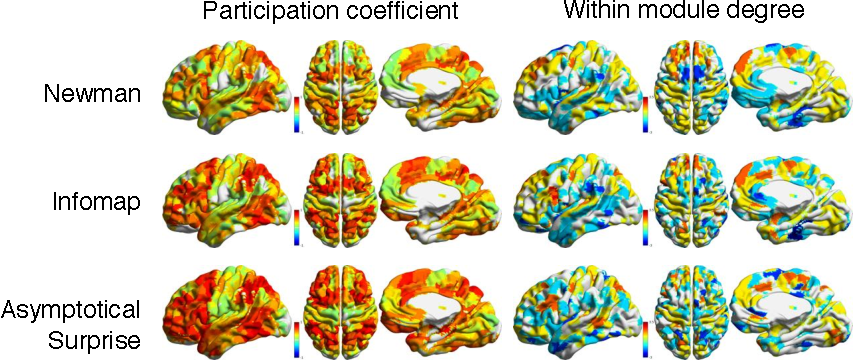
\includegraphics[width=\textwidth]{images/pacopaperfigure8.pdf}
% \caption{Anatomical distributions of the participation coefficient and within-module degree z-score for the resting state functional connectivity network partitioned by the three community detection methods.}
% \label{fig:hubclassification}
% \end{figure}


% \begin{figure}[htb!]
% 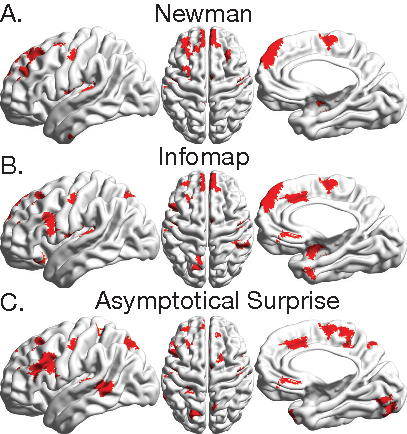
\includegraphics[width=\textwidth]{images/pacopaperfigure9.pdf}
% \caption{Nodes presenting simultaneously large values of the participation coefficient and within-module degree (larger than 0.6 and 1.5, respectively) for the three community detection methods. These nodes are thought to represent the connector hubs responsible for the integration of the networks's modules.
% }
% \label{fig:hubclassification_threshold}
% \end{figure}

% \subsection{Validation of Asymptotical Surprise in model networks}
% The performance of Asymptotical Surprise optimization by PACO was assessed in model graphs with a built-in community structure, and compared with two established community detection methods. We have chosen two synthetic benchmark networks, the ring of cliques and the LFR network.

% The ring of cliques presents a clear-cut modular structure by construct, with modules corresponding to complete subgraphs of variable sizes sampled from a power-law distribution. 
% This toy network proved useful to assess the effects of the resolution limit in the presence of a wide distribution of cluster sizes. The effects of this limit were particularly apparent for Newman's Modularity (Figure~\ref{fig:nmisensitivityspecificityringclique}), that showed poor Sensitivity even for noiseless rings of cliques, plateauing at a value of $0.75$.
% This is consistent with the findings of~\cite{fortunato2007}, that showed that for Modularity the resolution limit is set by the square root of the total number of edges in the graph.
% For Infomap, this limit is less severe and is determined by the number of inter-cluster edges~\cite{kawamoto2015}. Accordingly, the effects of the resolution limit were not apparent in this model network, where modules are sparingly connected by single edges.
% Asymptotical Surprise presented the best performance, consistent with the idea that this cost function is quasi-resolution limit free~\cite{traag2015}.

% However, real brain networks are characterized by heterogeneous distributions of node degree, with fat tails and power-law decays~\cite{bullmore2009}. Such heterogeneity is critical, as it determines some of the remarkable features of brain connectivity networks, including resilience to random failure and rich-clubness~\cite{vandenheuvel2011,vandenheuvel2013a}. To provide a more realistic benchmark, we used the Lancichinetti-Fortunato-Radicchi algorithm~\cite{lancichinetti2008}, that makes it possible to generate networks with realistic and tunable power law degree distribution and community sizes.

% For LFR networks, the difference in performance in the low-noise regime was more nuanced for the three methods compared in this study, possibly a result of a fuzzier community structure of the LFR network compared to the ring of cliques, and of the narrower distribution of cluster sizes. However, the picture appears different when noise and intersubject variability were injected into the network structure.

% Noise and other sources of variability in the data can significantly affect the structure of the resulting network representation.
% Noisy fMRI time-courses, for example, may introduce spurious correlations in brain functional connectivity networks.
% This problem may be particularly relevant for methods endowed with high resolution, like Asymptotical Surprise, that may be more vulnerable to False Positives generated by the mis-assignment of peripheral nodes, particularly in small clusters. Hence, the resolving power of community detection methods should be gauged against Specificity, which may be affected by noise in the distribution of edges that define the network's structure.
% However, to the best of our knowledge, this aspect has never been considered in the existing literature assessing the performance of community detection algorithms as applied to the study of brain connectivity.

% To this end, we have devised methods to inject noise, with amplitude and spectral distribution that mimic those of experimental noise, into networks with a well defined planted structure. Moreover, we have generated different instances for each network, corresponding to different subjects in a group, to account for intersubject variability that occurs in typical neuroimaging studies. 

% Unsurprisingly, for all methods and networks, detection of the planted structure improved with decreasing levels of noise, and with increasing number of subjects in the study.
% However, Asymptotical Surprise appeared to provide a superior performance in terms of NMI and Sensitivity to the planted structure for lower SNRs in both types of networks, while its Specificity was in line with that of resolution-limited methods like Newman's and Infomap (Figures \ref{fig:nmisensitivityspecificityringclique},\ref{fig:nmisensitivityspecificitylfr}).
% This rules out the idea that the higher sensitivity to small clusters of Asymptotical Surprise may be detrimental in noisy networks, making it more vulnerable to small, spurious modules.

% \subsection{Asymptotical Surprise optimization on resting state networks}
% Application of Asymptotical Surprise maximization to a group-level, resting state functional connectivity network from the brains of $27$ healthy subjects revealed a heterogeneous distribution of modules, with large and small modules coexisting in the optimal partition.
% This is in keeping with previous findings with binary Surprise~\cite{nicolini2016}.
% These modules closely reflect functional networks reported in many studies using Independent Component Analysis or other multivariate methods, including the sensorimotor, visual, default mode, executive, and attentional networks.
% Moreover, anatomically defined subcortical structures, like the hippocampus and parahippocampal formations emerged as independent moduli.

% While this is entirely consistent with our understanding of the neurofunctional and anatomical organization of the human brain, the accuracy of Asymptotical Surprise in identifying these networks is notable.
% Indeed, Surprise, like other graph-based community detection methods, divides networks into disjoint clusters of nodes on the basis of topological criteria.
% While a correspondence between topological modularity and functional networks identified by, e.g. Independent Component Analysis, may be expected, it is not a given, for they are defined on different principles. Indeed, multivariate methods like ICA separate components on the basis of the statistical independence of the time-courses, and do not convey information regarding the mutual relationship between modules nor about their topological organization.

% Previous studies applying resolution-limited methods like Newman's Modularity to the same dataset hereby analyzed~\cite{crossley2013a} found a few, large modules encompassing large-scale networks, but failed to identify finer, neurofunctionally plausible substructures like those shown in the present study. Infomap, on the other hand, proved sensitive to heterogeneously distributed clusters, thus implying that this method does not have an intrinsic scale, like Modularity and variations thereof based on the introduction of a resolution parameter. 
% However, Asymptotical Surprise appears to provide superior performance in identifying small subnetworks, particularly in the presence of noise, thus suggesting that this method may represent a new standard for community detection in brain networks. It should also be noted that no symmetry constraint was imposed, and the symmetrical bilateral distribution of nodes in the retrieved modules arises entirely from Asymptotical Surprise optimization. 

% Hierarchical clustering methods have been extensively applied to investigate the structure of brain connectivity networks, showing smaller and smaller clusters as the modules are iteratively subdivided~\cite{meunier2010}. Maximization of Asymptotical Surprise reflects the optimal cut through the dendrogram representing connectivity at these different levels of subdivision, and provides information on the optimal partition of the network. Hence, the heterogeneous distribution of cluster sizes retrieved by Asymptotical Surprise suggests that multiple scales of structure exist at the same level of the dendrogram.

% Finally, abnormal functional connectivity has been observed in a number of neurological and psychiatric diseases, but the coarse resolution of methods like Newman's Modularity~\cite{fornito2015} may have not detected differences in the modular organization of networks in patients compared to healthy controls. The improved resolution and sensitivity to multiscale structure afforded by Asymptotical Surprise may provide a powerful means to assess the brain functional architecture in disease states, thus contributing a potential imaging-based marker and a key to interpret the functional effects of aberrant connectivity.
% \subsection{Hub classification}
% The presence of heterogeneously distributed modules in functional connectivity networks may have important consequences for our understanding of the brain functional organization. By way of example, it has been shown that highly connected nodes, or hubs, are critically important in brain connectivity networks, and may play different roles depending on their position and connectivity distribution within and between modules~\cite{bullmore2009}. Hubs that primarily connect to nodes within the same community are dubbed “provincial hubs”, and are thought to be responsible for the definition and stability of the modules. Conversely, hubs that connect different modules are referred to as “connector hubs” and ensure integration of the activity of the network. The classification of hubs strongly depends on the modular structure that is considered, and inaccurate partitioning due to the resolution limit can lead to the wrong interpretation of their role in the interplay between segregation and integration of brain function~\cite{bullmore2009}. The present study suggests that this may have been the case in previous studies, in which resolution limited methods characterized by an intrinsic scale have been used, and provides a solution that may enable more accurate classification of hubs and nodes.

% The connector hubs identified by our three methods (Asymptotical Surprise, InfoMap and Newman) present some substantial differences, consistent with the idea that hub classification depends on community structure. These differences are particularly interesting in the light of the important role that connector hubs are thought to play in integrating information flow through the brain, and their putative role in brain disease \cite{crossley2014,stam2014}. By way of example, the Precuneus and the Cingulate Cortex are highlighted by Asymptotical Surprise, but not by Newman's Modularity, as connector hubs. These are two key elements of the Default Mode Network that have been consistently identified as vulnerable regions in neurological diseases~\cite{vandenheuvel2013a,buckner2009}. 
% Community detection by resolution limited free methods should enable more accurate classification of hub nodes, and improve our understanding of their role in brain disease. 

% \subsection{Limitations of Asymptotical Surprise}
% Some caution should be taken in the interpretation of the graphs in Figures \ref{fig:nmisensitivityspecificityringclique} and \ref{fig:nmisensitivityspecificitylfr}.
% Indeed, the SNRs of the synthetic networks we have generated reflect noise with features, like a Rician distribution, that mimic some, but not all aspects of the variability of experimental data.
% By way of example, the brain parcellation scheme applied to define the nodes, and the heterogeneity of voxels within these parcels, may play a role that is difficult to model in toy networks~\cite{fornito2010}.
% Hence, the simulated Sensitivity and Specificity as a function of SNR and number of subjects should not be taken as absolute values to be used in the power and sample size estimation in real experimental designs.
% Nevertheless, these simulations provide useful information on the dependence of these parameters on noise levels, and a rigorous means to assess the relative merits of different community detection methods.

% Finally, we should note that the maximum value of Asymptotical Surprise calculated with PACO is an index of quality of the entire partition, and not of individual modules.
% Hence, individual modules may not all have the same strength of internal cohesiveness relative to their connection with other modules.
% We have found hints of this phenomenon in the comparison of nearly-optimal partitions obtained in the $10,000$ runs of PACO that we have performed to find the optimal community structure for this network.
% The overall community structure appeared to be robust, with most modules persistently emerging in every nearly-optimal partition, but in some cases we observed pairs of modules splitting or merging in otherwise similar solutions. Most notably, this was observed for the thalamus that in some instances was merged with the basal cluster and in others, featured as a separate module.
% This phenomenon may be less critical for methods like Newman's Modularity that have an intrinsic scale and retrieve uniformly distributed modules.

% \section{Conclusions}
% We have extended the use of Surprise, a resolution-limit-free fitness function for the study of the modular structure of complex networks, to weighted brain functional connectivity networks. Specifically, we have developed a novel method, dubbed PACO, for the optimization of Asymptotical Surprise, a weighted counterpart of Surprise in the limit of large networks. We have applied PACO optimization of Asymptotical Surprise in synthetic networks to evaluate the relative merits of this novel approach against Newman's Modularity and Infomap, two of the leading methods used for community detection in brain connectivity networks. Specifically, we have implemented a process to inject noise into networks endowed with a ground-truth modular structure to assess the trade-off between improved resolution afforded by Asymptotical Surprise and potential sensitivity to spurious correlations introduced by variability in the data. Asymptotical Surprise optimization proved superior to existing methods in terms of Sensitivity and accuracy in detection of the planted structure as measured by Normalized Mutual Information, while showing comparable Specificity. We have also applied our approach to the partitioning of functional connectivity networks from resting state fMRI experiments. Direct comparison with other methods clearly demonstrated improved capability to identify neurofunctionally plausible and anatomically well-defined substructures otherwise concealed by the resolution limit. Asymptotical Surprise revealed a complex modular structure of resting state connectivity, with communities of widely different sizes reflecting distributed functional networks alongside with small, anatomically or functionally defined modules. This evidence corroborates the idea that the resolution limit may have negatively affected current models of the brain modular organization and the identification of the hubs responsible for integration of functional modules. 
% The application of methods like Asymptotical Surprise provides a novel, powerful approach to study the modular structure of brain connectivity beyond this limit.
